\documentclass[14pt]{beamer}
\usetheme{defense}
\graphicspath{{../../figures/}}

\newcommand{\leftRect}[2]{\node[draw=text,very thick,rounded corners, text width=0.46\textwidth,minimum height=6cm] at (0,0) {\centering\textbf{#1}\\ \raggedright \color{text}#2};}
\newcommand{\rightRect}[2]{\node[draw=text,very thick,rounded corners, text width=0.46\textwidth,minimum height=6cm] at (0.54\textwidth,0) {\centering\textbf{#1}\\ \raggedright \color{text}#2};}

\usepackage{tikz}
\usepackage{svg}
\setcounter{tocdepth}{1}

\title{Memristors-based recurent modules for neural computing}

\subtitle{}

\newcommand {\Supervisor} {
  {Dr. Diogo Caetano} and {Dr. Ruxandra Barbulescu}}
\newcommand {\CommitteeMembers} {
  {Prof./Dr. Lorem Ipsum}}
\newcommand {\Chairperson} {{Prof./Dr. Lorem Ipsum}}
\author[V. BARBAZA]{{Valentin BARBAZA}}

\date{17 november 2023}

\logo{
  \begin{tikzpicture}[overlay,remember picture]
    \node[left=0cm] at (current page.33){
      
\includegraphics[height=1cm]{logos/inesc-mn.png}
      \hspace{1pt}
      
\includegraphics[height=1cm]{logos/ist.eps}
      
\includegraphics[height=1cm]{logos/inesc-id.eps}
    };
  \end{tikzpicture}
}

\begin{document}

\frame{\titlepage}

\begin{frame}
  \frametitle{Table of Contents}
  \tableofcontents
\end{frame}

\section{Motivation and objectives}

\begin{frame}{\insertsection}
  \begin{columns}
    \column{.6\textwidth}
    \begin{itemize}
      \item NNs complexity grows rapidly
      \item So does its computation time
    \end{itemize}
    \column{.4\textwidth}
    \includesvg[width=\columnwidth,pretex=\scriptsize]{NN_explained.svg}
  \end{columns}
\end{frame}

\begin{frame}{\insertsection}
  \begin{columns}
    \column{.6\textwidth}
    \begin{itemize}
      \item Reduce computation by using analog
      \item Allows use for time sensitive problems
    \end{itemize}
    \column{.4\textwidth}
    \includesvg[width=\columnwidth,pretex=\scriptsize]{NN_explained.svg}
  \end{columns}
\end{frame}

\section{Introduction}

\begin{frame}{\insertsection}{RNNs}
  RNNs are a type of NN :
  \begin{itemize}
    \item Used for time dependent data
    \item That have a feedback connection
  \end{itemize}

  \begin{equation}\label{eq:rnn}
    \overrightarrow{h_t}=f(\overrightarrow{x_t},\overrightarrow{h_{t-1}})
  \end{equation}
\end{frame}

\begin{frame}{\insertsection}{LSTMs}
  \includesvg[width=\columnwidth,pretex=\scriptsize]{lstm/lstmCell}
\end{frame}

\begin{frame}{\insertsection}{GRUs}
  \includesvg[width=\columnwidth,pretex=\scriptsize]{gru/encoderCell}
\end{frame}

\begin{frame}{\insertsection}{Memristors}
  \begin{columns}
    \column{.65\textwidth}
    \includesvg[width=\columnwidth,pretex=\tiny]{memristor/memristor}
    \column{.4\textwidth}
    \begin{itemize}
      \item Recent electical component
      \item Variable resistance
    \end{itemize}
  \end{columns}
\end{frame}


\section{The circuits}
\subsection{Activation functions}
\begin{frame}{\insertsection}{\insertsubsection}
  \begin{columns}
    \column{.7\textwidth}
    \includesvg[width=\columnwidth,pretex=\scriptsize]{activation/afCircuit}
    \column{.4\textwidth}
    \begin{itemize}
      \item Creates analog activation functions
      \item Is used for both tanh and sigmoid activation functions
    \end{itemize}
  \end{columns}
\end{frame}

\begin{frame}{\insertsection}{\insertsubsection}
  \begin{center}
    \includesvg[width=0.75\columnwidth,pretex=\tiny]{activation/afGraph}
  \end{center}
\end{frame}

\subsection{Memory cell}

\begin{frame}{\insertsection}{\insertsubsection}
  \begin{columns}
    \column{.65\textwidth}
    \includesvg[width=\columnwidth,pretex=\tiny]{memcell/memCircuit}
    \column{.4\textwidth}
    \begin{itemize}
      \item Stores analog value
      \item Has two CMOS switches to avoid leakage
    \end{itemize}
  \end{columns}
\end{frame}

\begin{frame}{\insertsection}{\insertsubsection}
  \begin{center}
    \includesvg[width=.75\columnwidth,pretex=\tiny]{memcell/data-loss}
  \end{center}
\end{frame}

\section{The tools}
\begin{frame}{\insertsection}{\insertsubsection}
  So far, I have designed some smaller elements required for the system to work such as the activation function for example.\\
  I've designed a full size LSTM (with 4 hidden state).
  \begin{figure}
    \centering
    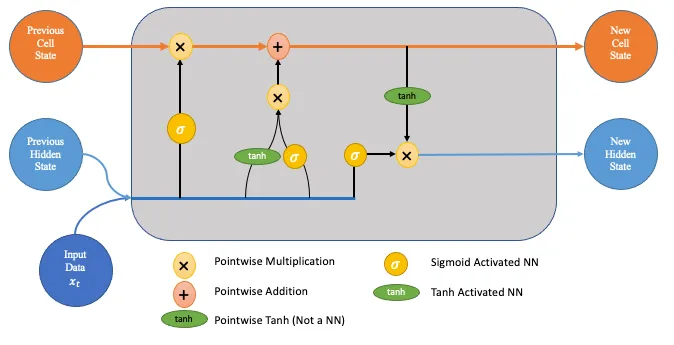
\includegraphics[height=0.35\textheight]{lstm/lstm.png}
  \end{figure}
  I am now working on a way to generate LSTM network of any size.
\end{frame}

\section{The datasets}
\begin{frame}{\insertsection}{\insertsubsection}
  I now need to run the simulations and compare the results of my simulation with the results a digital LSTM (running with Keras for example).
\end{frame}

\subsection{Tressk}
\begin{frame}{jdjd}{}
\end{frame}

\end{document}
